% Created by tikzDevice version 0.12 on 2019-04-10 16:32:26
% !TEX encoding = UTF-8 Unicode
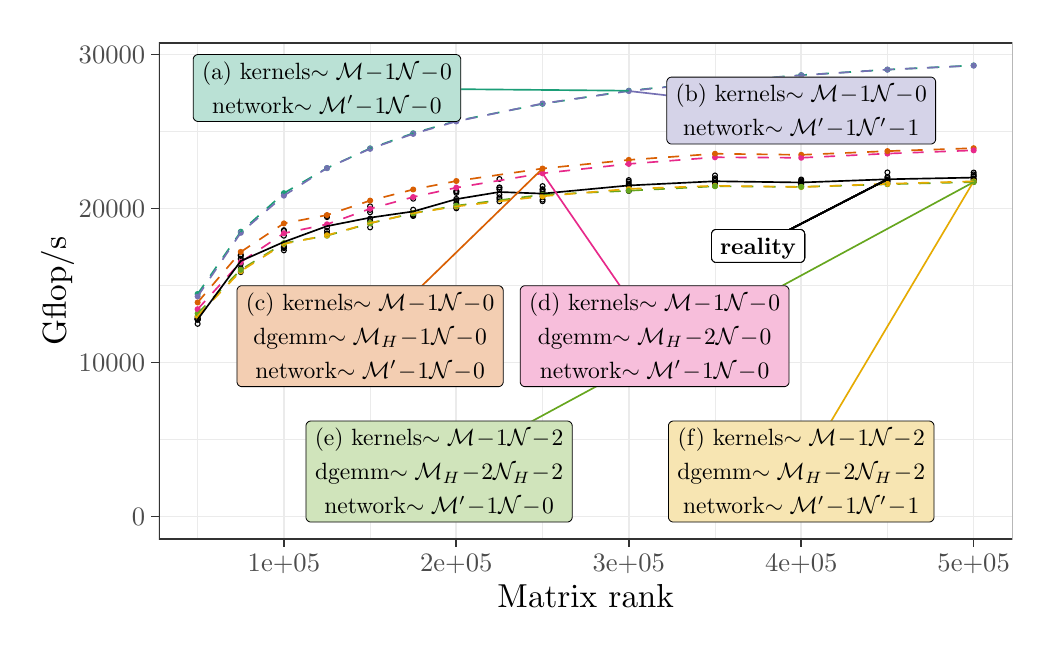
\begin{tikzpicture}[x=1pt,y=1pt]
\definecolor{fillColor}{RGB}{255,255,255}
\path[use as bounding box,fill=fillColor,fill opacity=0.00] (0,0) rectangle (361.35,216.81);
\begin{scope}
\path[clip] (  0.00,  0.00) rectangle (361.35,216.81);
\definecolor{drawColor}{RGB}{255,255,255}
\definecolor{fillColor}{RGB}{255,255,255}

\path[draw=drawColor,line width= 0.6pt,line join=round,line cap=round,fill=fillColor] (  0.00,  0.00) rectangle (361.35,216.81);
\end{scope}
\begin{scope}
\path[clip] ( 47.40, 31.96) rectangle (355.85,211.31);
\definecolor{fillColor}{RGB}{255,255,255}

\path[fill=fillColor] ( 47.40, 31.96) rectangle (355.85,211.31);
\definecolor{drawColor}{gray}{0.92}

\path[draw=drawColor,line width= 0.3pt,line join=round] ( 47.40, 67.96) --
	(355.85, 67.96);

\path[draw=drawColor,line width= 0.3pt,line join=round] ( 47.40,123.64) --
	(355.85,123.64);

\path[draw=drawColor,line width= 0.3pt,line join=round] ( 47.40,179.33) --
	(355.85,179.33);

\path[draw=drawColor,line width= 0.3pt,line join=round] ( 61.42, 31.96) --
	( 61.42,211.31);

\path[draw=drawColor,line width= 0.3pt,line join=round] (123.74, 31.96) --
	(123.74,211.31);

\path[draw=drawColor,line width= 0.3pt,line join=round] (186.05, 31.96) --
	(186.05,211.31);

\path[draw=drawColor,line width= 0.3pt,line join=round] (248.36, 31.96) --
	(248.36,211.31);

\path[draw=drawColor,line width= 0.3pt,line join=round] (310.67, 31.96) --
	(310.67,211.31);

\path[draw=drawColor,line width= 0.6pt,line join=round] ( 47.40, 40.12) --
	(355.85, 40.12);

\path[draw=drawColor,line width= 0.6pt,line join=round] ( 47.40, 95.80) --
	(355.85, 95.80);

\path[draw=drawColor,line width= 0.6pt,line join=round] ( 47.40,151.48) --
	(355.85,151.48);

\path[draw=drawColor,line width= 0.6pt,line join=round] ( 47.40,207.17) --
	(355.85,207.17);

\path[draw=drawColor,line width= 0.6pt,line join=round] ( 92.58, 31.96) --
	( 92.58,211.31);

\path[draw=drawColor,line width= 0.6pt,line join=round] (154.89, 31.96) --
	(154.89,211.31);

\path[draw=drawColor,line width= 0.6pt,line join=round] (217.20, 31.96) --
	(217.20,211.31);

\path[draw=drawColor,line width= 0.6pt,line join=round] (279.52, 31.96) --
	(279.52,211.31);

\path[draw=drawColor,line width= 0.6pt,line join=round] (341.83, 31.96) --
	(341.83,211.31);
\definecolor{drawColor}{RGB}{0,0,0}

\path[draw=drawColor,line width= 0.4pt,line join=round,line cap=round] (341.83,164.46) circle (  0.89);

\path[draw=drawColor,line width= 0.4pt,line join=round,line cap=round] ( 61.42,111.28) circle (  0.89);

\path[draw=drawColor,line width= 0.4pt,line join=round,line cap=round] (217.20,157.83) circle (  0.89);

\path[draw=drawColor,line width= 0.4pt,line join=round,line cap=round] (279.52,160.73) circle (  0.89);

\path[draw=drawColor,line width= 0.4pt,line join=round,line cap=round] (123.74,150.98) circle (  0.89);

\path[draw=drawColor,line width= 0.4pt,line join=round,line cap=round] (186.05,154.66) circle (  0.89);

\path[draw=drawColor,line width= 0.4pt,line join=round,line cap=round] (310.67,162.84) circle (  0.89);

\path[draw=drawColor,line width= 0.4pt,line join=round,line cap=round] (248.36,163.40) circle (  0.89);

\path[draw=drawColor,line width= 0.4pt,line join=round,line cap=round] (154.89,154.94) circle (  0.89);

\path[draw=drawColor,line width= 0.4pt,line join=round,line cap=round] ( 92.58,143.35) circle (  0.89);

\path[draw=drawColor,line width= 0.4pt,line join=round,line cap=round] ( 77.00,134.72) circle (  0.89);

\path[draw=drawColor,line width= 0.4pt,line join=round,line cap=round] (108.16,148.37) circle (  0.89);

\path[draw=drawColor,line width= 0.4pt,line join=round,line cap=round] (170.47,159.11) circle (  0.89);

\path[draw=drawColor,line width= 0.4pt,line join=round,line cap=round] ( 77.00,134.56) circle (  0.89);

\path[draw=drawColor,line width= 0.4pt,line join=round,line cap=round] (217.20,161.73) circle (  0.89);

\path[draw=drawColor,line width= 0.4pt,line join=round,line cap=round] (310.67,164.51) circle (  0.89);

\path[draw=drawColor,line width= 0.4pt,line join=round,line cap=round] (154.89,157.78) circle (  0.89);

\path[draw=drawColor,line width= 0.4pt,line join=round,line cap=round] (139.31,148.92) circle (  0.89);

\path[draw=drawColor,line width= 0.4pt,line join=round,line cap=round] ( 61.42,111.34) circle (  0.89);

\path[draw=drawColor,line width= 0.4pt,line join=round,line cap=round] (170.47,162.12) circle (  0.89);

\path[draw=drawColor,line width= 0.4pt,line join=round,line cap=round] (186.05,158.44) circle (  0.89);

\path[draw=drawColor,line width= 0.4pt,line join=round,line cap=round] (108.16,142.13) circle (  0.89);

\path[draw=drawColor,line width= 0.4pt,line join=round,line cap=round] (123.74,147.81) circle (  0.89);

\path[draw=drawColor,line width= 0.4pt,line join=round,line cap=round] ( 92.58,143.63) circle (  0.89);

\path[draw=drawColor,line width= 0.4pt,line join=round,line cap=round] (341.83,163.23) circle (  0.89);

\path[draw=drawColor,line width= 0.4pt,line join=round,line cap=round] (279.52,161.95) circle (  0.89);

\path[draw=drawColor,line width= 0.4pt,line join=round,line cap=round] (248.36,159.89) circle (  0.89);

\path[draw=drawColor,line width= 0.4pt,line join=round,line cap=round] ( 61.42,111.61) circle (  0.89);

\path[draw=drawColor,line width= 0.4pt,line join=round,line cap=round] (108.16,141.96) circle (  0.89);

\path[draw=drawColor,line width= 0.4pt,line join=round,line cap=round] (341.83,161.40) circle (  0.89);

\path[draw=drawColor,line width= 0.4pt,line join=round,line cap=round] (170.47,154.88) circle (  0.89);

\path[draw=drawColor,line width= 0.4pt,line join=round,line cap=round] (123.74,150.09) circle (  0.89);

\path[draw=drawColor,line width= 0.4pt,line join=round,line cap=round] (279.52,161.17) circle (  0.89);

\path[draw=drawColor,line width= 0.4pt,line join=round,line cap=round] ( 77.00,129.88) circle (  0.89);

\path[draw=drawColor,line width= 0.4pt,line join=round,line cap=round] (217.20,159.61) circle (  0.89);

\path[draw=drawColor,line width= 0.4pt,line join=round,line cap=round] (248.36,161.45) circle (  0.89);

\path[draw=drawColor,line width= 0.4pt,line join=round,line cap=round] (310.67,162.45) circle (  0.89);

\path[draw=drawColor,line width= 0.4pt,line join=round,line cap=round] (186.05,155.77) circle (  0.89);

\path[draw=drawColor,line width= 0.4pt,line join=round,line cap=round] (154.89,157.11) circle (  0.89);

\path[draw=drawColor,line width= 0.4pt,line join=round,line cap=round] ( 92.58,137.17) circle (  0.89);

\path[draw=drawColor,line width= 0.4pt,line join=round,line cap=round] (139.31,149.20) circle (  0.89);

\path[draw=drawColor,line width= 0.4pt,line join=round,line cap=round] (186.05,157.50) circle (  0.89);

\path[draw=drawColor,line width= 0.4pt,line join=round,line cap=round] ( 61.42,109.78) circle (  0.89);

\path[draw=drawColor,line width= 0.4pt,line join=round,line cap=round] (217.20,159.56) circle (  0.89);

\path[draw=drawColor,line width= 0.4pt,line join=round,line cap=round] (108.16,142.46) circle (  0.89);

\path[draw=drawColor,line width= 0.4pt,line join=round,line cap=round] ( 92.58,137.90) circle (  0.89);

\path[draw=drawColor,line width= 0.4pt,line join=round,line cap=round] (341.83,163.79) circle (  0.89);

\path[draw=drawColor,line width= 0.4pt,line join=round,line cap=round] ( 77.00,133.33) circle (  0.89);

\path[draw=drawColor,line width= 0.4pt,line join=round,line cap=round] (123.74,146.42) circle (  0.89);

\path[draw=drawColor,line width= 0.4pt,line join=round,line cap=round] (154.89,154.43) circle (  0.89);

\path[draw=drawColor,line width= 0.4pt,line join=round,line cap=round] (279.52,161.17) circle (  0.89);

\path[draw=drawColor,line width= 0.4pt,line join=round,line cap=round] (170.47,156.50) circle (  0.89);

\path[draw=drawColor,line width= 0.4pt,line join=round,line cap=round] (310.67,160.56) circle (  0.89);

\path[draw=drawColor,line width= 0.4pt,line join=round,line cap=round] (139.31,149.42) circle (  0.89);

\path[draw=drawColor,line width= 0.4pt,line join=round,line cap=round] (248.36,160.84) circle (  0.89);

\path[draw=drawColor,line width= 0.4pt,line join=round,line cap=round] (154.89,152.04) circle (  0.89);

\path[draw=drawColor,line width= 0.4pt,line join=round,line cap=round] (310.67,161.40) circle (  0.89);

\path[draw=drawColor,line width= 0.4pt,line join=round,line cap=round] (139.31,151.04) circle (  0.89);

\path[draw=drawColor,line width= 0.4pt,line join=round,line cap=round] (279.52,159.61) circle (  0.89);

\path[draw=drawColor,line width= 0.4pt,line join=round,line cap=round] (186.05,156.61) circle (  0.89);

\path[draw=drawColor,line width= 0.4pt,line join=round,line cap=round] ( 61.42,112.28) circle (  0.89);

\path[draw=drawColor,line width= 0.4pt,line join=round,line cap=round] (217.20,160.00) circle (  0.89);

\path[draw=drawColor,line width= 0.4pt,line join=round,line cap=round] (341.83,161.06) circle (  0.89);

\path[draw=drawColor,line width= 0.4pt,line join=round,line cap=round] ( 77.00,134.33) circle (  0.89);

\path[draw=drawColor,line width= 0.4pt,line join=round,line cap=round] (108.16,148.81) circle (  0.89);

\path[draw=drawColor,line width= 0.4pt,line join=round,line cap=round] (123.74,152.26) circle (  0.89);

\path[draw=drawColor,line width= 0.4pt,line join=round,line cap=round] ( 92.58,136.34) circle (  0.89);

\path[draw=drawColor,line width= 0.4pt,line join=round,line cap=round] (170.47,155.49) circle (  0.89);

\path[draw=drawColor,line width= 0.4pt,line join=round,line cap=round] (248.36,159.72) circle (  0.89);

\path[draw=drawColor,line width= 0.4pt,line join=round,line cap=round] (341.83,161.95) circle (  0.89);

\path[draw=drawColor,line width= 0.4pt,line join=round,line cap=round] ( 61.42,111.39) circle (  0.89);

\path[draw=drawColor,line width= 0.4pt,line join=round,line cap=round] (217.20,157.89) circle (  0.89);

\path[draw=drawColor,line width= 0.4pt,line join=round,line cap=round] (279.52,160.50) circle (  0.89);

\path[draw=drawColor,line width= 0.4pt,line join=round,line cap=round] (123.74,146.92) circle (  0.89);

\path[draw=drawColor,line width= 0.4pt,line join=round,line cap=round] (186.05,158.17) circle (  0.89);

\path[draw=drawColor,line width= 0.4pt,line join=round,line cap=round] (310.67,161.45) circle (  0.89);

\path[draw=drawColor,line width= 0.4pt,line join=round,line cap=round] (248.36,160.73) circle (  0.89);

\path[draw=drawColor,line width= 0.4pt,line join=round,line cap=round] (154.89,151.54) circle (  0.89);

\path[draw=drawColor,line width= 0.4pt,line join=round,line cap=round] ( 92.58,137.45) circle (  0.89);

\path[draw=drawColor,line width= 0.4pt,line join=round,line cap=round] ( 77.00,131.44) circle (  0.89);

\path[draw=drawColor,line width= 0.4pt,line join=round,line cap=round] (108.16,148.87) circle (  0.89);

\path[draw=drawColor,line width= 0.4pt,line join=round,line cap=round] (170.47,158.33) circle (  0.89);

\path[draw=drawColor,line width= 0.4pt,line join=round,line cap=round] ( 77.00,128.49) circle (  0.89);

\path[draw=drawColor,line width= 0.4pt,line join=round,line cap=round] (217.20,161.17) circle (  0.89);

\path[draw=drawColor,line width= 0.4pt,line join=round,line cap=round] (310.67,161.17) circle (  0.89);

\path[draw=drawColor,line width= 0.4pt,line join=round,line cap=round] (154.89,153.38) circle (  0.89);

\path[draw=drawColor,line width= 0.4pt,line join=round,line cap=round] (139.31,154.99) circle (  0.89);

\path[draw=drawColor,line width= 0.4pt,line join=round,line cap=round] ( 61.42,111.61) circle (  0.89);

\path[draw=drawColor,line width= 0.4pt,line join=round,line cap=round] (170.47,154.05) circle (  0.89);

\path[draw=drawColor,line width= 0.4pt,line join=round,line cap=round] (186.05,154.10) circle (  0.89);

\path[draw=drawColor,line width= 0.4pt,line join=round,line cap=round] (108.16,144.69) circle (  0.89);

\path[draw=drawColor,line width= 0.4pt,line join=round,line cap=round] (123.74,144.63) circle (  0.89);

\path[draw=drawColor,line width= 0.4pt,line join=round,line cap=round] ( 92.58,137.56) circle (  0.89);

\path[draw=drawColor,line width= 0.4pt,line join=round,line cap=round] (341.83,162.23) circle (  0.89);

\path[draw=drawColor,line width= 0.4pt,line join=round,line cap=round] (279.52,161.62) circle (  0.89);

\path[draw=drawColor,line width= 0.4pt,line join=round,line cap=round] (248.36,162.06) circle (  0.89);

\path[draw=drawColor,line width= 0.4pt,line join=round,line cap=round] ( 61.42,111.73) circle (  0.89);

\path[draw=drawColor,line width= 0.4pt,line join=round,line cap=round] (108.16,143.41) circle (  0.89);

\path[draw=drawColor,line width= 0.4pt,line join=round,line cap=round] (341.83,163.01) circle (  0.89);

\path[draw=drawColor,line width= 0.4pt,line join=round,line cap=round] (170.47,158.95) circle (  0.89);

\path[draw=drawColor,line width= 0.4pt,line join=round,line cap=round] (123.74,146.19) circle (  0.89);

\path[draw=drawColor,line width= 0.4pt,line join=round,line cap=round] (279.52,160.23) circle (  0.89);

\path[draw=drawColor,line width= 0.4pt,line join=round,line cap=round] ( 77.00,133.16) circle (  0.89);

\path[draw=drawColor,line width= 0.4pt,line join=round,line cap=round] (217.20,160.50) circle (  0.89);

\path[draw=drawColor,line width= 0.4pt,line join=round,line cap=round] (248.36,162.40) circle (  0.89);

\path[draw=drawColor,line width= 0.4pt,line join=round,line cap=round] (310.67,161.84) circle (  0.89);

\path[draw=drawColor,line width= 0.4pt,line join=round,line cap=round] (186.05,159.56) circle (  0.89);

\path[draw=drawColor,line width= 0.4pt,line join=round,line cap=round] (154.89,157.55) circle (  0.89);

\path[draw=drawColor,line width= 0.4pt,line join=round,line cap=round] ( 92.58,141.63) circle (  0.89);

\path[draw=drawColor,line width= 0.4pt,line join=round,line cap=round] (139.31,148.76) circle (  0.89);
\definecolor{drawColor}{RGB}{230,171,2}
\definecolor{fillColor}{RGB}{230,171,2}

\path[draw=drawColor,line width= 0.4pt,line join=round,line cap=round,fill=fillColor] ( 77.00,128.82) circle (  0.89);

\path[draw=drawColor,line width= 0.4pt,line join=round,line cap=round,fill=fillColor] (139.31,149.76) circle (  0.89);

\path[draw=drawColor,line width= 0.4pt,line join=round,line cap=round,fill=fillColor] (248.36,159.67) circle (  0.89);
\definecolor{drawColor}{RGB}{217,95,2}
\definecolor{fillColor}{RGB}{217,95,2}

\path[draw=drawColor,line width= 0.4pt,line join=round,line cap=round,fill=fillColor] ( 61.42,117.52) circle (  0.89);

\path[draw=drawColor,line width= 0.4pt,line join=round,line cap=round,fill=fillColor] (123.74,154.32) circle (  0.89);

\path[draw=drawColor,line width= 0.4pt,line join=round,line cap=round,fill=fillColor] (217.20,169.02) circle (  0.89);

\path[draw=drawColor,line width= 0.4pt,line join=round,line cap=round,fill=fillColor] (341.83,173.26) circle (  0.89);
\definecolor{drawColor}{RGB}{230,171,2}
\definecolor{fillColor}{RGB}{230,171,2}

\path[draw=drawColor,line width= 0.4pt,line join=round,line cap=round,fill=fillColor] ( 92.58,138.68) circle (  0.89);

\path[draw=drawColor,line width= 0.4pt,line join=round,line cap=round,fill=fillColor] (154.89,152.21) circle (  0.89);

\path[draw=drawColor,line width= 0.4pt,line join=round,line cap=round,fill=fillColor] (279.52,159.22) circle (  0.89);

\path[draw=drawColor,line width= 0.4pt,line join=round,line cap=round,fill=fillColor] ( 61.42,112.62) circle (  0.89);

\path[draw=drawColor,line width= 0.4pt,line join=round,line cap=round,fill=fillColor] (123.74,146.19) circle (  0.89);

\path[draw=drawColor,line width= 0.4pt,line join=round,line cap=round,fill=fillColor] (217.20,158.56) circle (  0.89);

\path[draw=drawColor,line width= 0.4pt,line join=round,line cap=round,fill=fillColor] (341.83,161.28) circle (  0.89);
\definecolor{drawColor}{RGB}{231,41,138}
\definecolor{fillColor}{RGB}{231,41,138}

\path[draw=drawColor,line width= 0.4pt,line join=round,line cap=round,fill=fillColor] ( 77.00,132.11) circle (  0.89);

\path[draw=drawColor,line width= 0.4pt,line join=round,line cap=round,fill=fillColor] (139.31,155.60) circle (  0.89);

\path[draw=drawColor,line width= 0.4pt,line join=round,line cap=round,fill=fillColor] (248.36,169.97) circle (  0.89);
\definecolor{drawColor}{RGB}{102,166,30}
\definecolor{fillColor}{RGB}{102,166,30}

\path[draw=drawColor,line width= 0.4pt,line join=round,line cap=round,fill=fillColor] ( 61.42,113.56) circle (  0.89);

\path[draw=drawColor,line width= 0.4pt,line join=round,line cap=round,fill=fillColor] (123.74,146.14) circle (  0.89);

\path[draw=drawColor,line width= 0.4pt,line join=round,line cap=round,fill=fillColor] (217.20,157.89) circle (  0.89);

\path[draw=drawColor,line width= 0.4pt,line join=round,line cap=round,fill=fillColor] (341.83,161.01) circle (  0.89);
\definecolor{drawColor}{RGB}{231,41,138}
\definecolor{fillColor}{RGB}{231,41,138}

\path[draw=drawColor,line width= 0.4pt,line join=round,line cap=round,fill=fillColor] ( 61.42,115.07) circle (  0.89);

\path[draw=drawColor,line width= 0.4pt,line join=round,line cap=round,fill=fillColor] (123.74,151.37) circle (  0.89);

\path[draw=drawColor,line width= 0.4pt,line join=round,line cap=round,fill=fillColor] (217.20,167.58) circle (  0.89);

\path[draw=drawColor,line width= 0.4pt,line join=round,line cap=round,fill=fillColor] (341.83,172.48) circle (  0.89);

\path[draw=drawColor,line width= 0.4pt,line join=round,line cap=round,fill=fillColor] (108.16,145.75) circle (  0.89);

\path[draw=drawColor,line width= 0.4pt,line join=round,line cap=round,fill=fillColor] (186.05,164.18) circle (  0.89);

\path[draw=drawColor,line width= 0.4pt,line join=round,line cap=round,fill=fillColor] (310.67,171.31) circle (  0.89);
\definecolor{drawColor}{RGB}{217,95,2}
\definecolor{fillColor}{RGB}{217,95,2}

\path[draw=drawColor,line width= 0.4pt,line join=round,line cap=round,fill=fillColor] ( 77.00,135.78) circle (  0.89);

\path[draw=drawColor,line width= 0.4pt,line join=round,line cap=round,fill=fillColor] (139.31,158.33) circle (  0.89);

\path[draw=drawColor,line width= 0.4pt,line join=round,line cap=round,fill=fillColor] (248.36,171.25) circle (  0.89);

\path[draw=drawColor,line width= 0.4pt,line join=round,line cap=round,fill=fillColor] (108.16,149.09) circle (  0.89);

\path[draw=drawColor,line width= 0.4pt,line join=round,line cap=round,fill=fillColor] (186.05,165.91) circle (  0.89);

\path[draw=drawColor,line width= 0.4pt,line join=round,line cap=round,fill=fillColor] (310.67,172.20) circle (  0.89);
\definecolor{drawColor}{RGB}{102,166,30}
\definecolor{fillColor}{RGB}{102,166,30}

\path[draw=drawColor,line width= 0.4pt,line join=round,line cap=round,fill=fillColor] (108.16,141.63) circle (  0.89);

\path[draw=drawColor,line width= 0.4pt,line join=round,line cap=round,fill=fillColor] (186.05,156.44) circle (  0.89);

\path[draw=drawColor,line width= 0.4pt,line join=round,line cap=round,fill=fillColor] (310.67,160.23) circle (  0.89);
\definecolor{drawColor}{RGB}{230,171,2}
\definecolor{fillColor}{RGB}{230,171,2}

\path[draw=drawColor,line width= 0.4pt,line join=round,line cap=round,fill=fillColor] (108.16,141.79) circle (  0.89);

\path[draw=drawColor,line width= 0.4pt,line join=round,line cap=round,fill=fillColor] (186.05,155.88) circle (  0.89);

\path[draw=drawColor,line width= 0.4pt,line join=round,line cap=round,fill=fillColor] (310.67,160.39) circle (  0.89);
\definecolor{drawColor}{RGB}{102,166,30}
\definecolor{fillColor}{RGB}{102,166,30}

\path[draw=drawColor,line width= 0.4pt,line join=round,line cap=round,fill=fillColor] ( 77.00,129.32) circle (  0.89);

\path[draw=drawColor,line width= 0.4pt,line join=round,line cap=round,fill=fillColor] (139.31,149.76) circle (  0.89);

\path[draw=drawColor,line width= 0.4pt,line join=round,line cap=round,fill=fillColor] (248.36,159.50) circle (  0.89);

\path[draw=drawColor,line width= 0.4pt,line join=round,line cap=round,fill=fillColor] ( 92.58,138.95) circle (  0.89);

\path[draw=drawColor,line width= 0.4pt,line join=round,line cap=round,fill=fillColor] (154.89,152.49) circle (  0.89);

\path[draw=drawColor,line width= 0.4pt,line join=round,line cap=round,fill=fillColor] (279.52,159.28) circle (  0.89);
\definecolor{drawColor}{RGB}{217,95,2}
\definecolor{fillColor}{RGB}{217,95,2}

\path[draw=drawColor,line width= 0.4pt,line join=round,line cap=round,fill=fillColor] ( 92.58,146.08) circle (  0.89);

\path[draw=drawColor,line width= 0.4pt,line join=round,line cap=round,fill=fillColor] (154.89,161.40) circle (  0.89);

\path[draw=drawColor,line width= 0.4pt,line join=round,line cap=round,fill=fillColor] (279.52,170.86) circle (  0.89);
\definecolor{drawColor}{RGB}{231,41,138}
\definecolor{fillColor}{RGB}{231,41,138}

\path[draw=drawColor,line width= 0.4pt,line join=round,line cap=round,fill=fillColor] ( 92.58,142.52) circle (  0.89);

\path[draw=drawColor,line width= 0.4pt,line join=round,line cap=round,fill=fillColor] (154.89,159.00) circle (  0.89);

\path[draw=drawColor,line width= 0.4pt,line join=round,line cap=round,fill=fillColor] (279.52,169.80) circle (  0.89);
\definecolor{drawColor}{RGB}{27,158,119}
\definecolor{fillColor}{RGB}{27,158,119}

\path[draw=drawColor,line width= 0.4pt,line join=round,line cap=round,fill=fillColor] (341.83,203.16) circle (  0.89);

\path[draw=drawColor,line width= 0.4pt,line join=round,line cap=round,fill=fillColor] ( 61.42,120.58) circle (  0.89);

\path[draw=drawColor,line width= 0.4pt,line join=round,line cap=round,fill=fillColor] (217.20,194.03) circle (  0.89);

\path[draw=drawColor,line width= 0.4pt,line join=round,line cap=round,fill=fillColor] (279.52,199.65) circle (  0.89);

\path[draw=drawColor,line width= 0.4pt,line join=round,line cap=round,fill=fillColor] (123.74,173.20) circle (  0.89);

\path[draw=drawColor,line width= 0.4pt,line join=round,line cap=round,fill=fillColor] (154.89,183.11) circle (  0.89);

\path[draw=drawColor,line width= 0.4pt,line join=round,line cap=round,fill=fillColor] ( 92.58,157.00) circle (  0.89);

\path[draw=drawColor,line width= 0.4pt,line join=round,line cap=round,fill=fillColor] (139.31,178.66) circle (  0.89);

\path[draw=drawColor,line width= 0.4pt,line join=round,line cap=round,fill=fillColor] (186.05,189.29) circle (  0.89);

\path[draw=drawColor,line width= 0.4pt,line join=round,line cap=round,fill=fillColor] (310.67,201.65) circle (  0.89);

\path[draw=drawColor,line width= 0.4pt,line join=round,line cap=round,fill=fillColor] (248.36,197.26) circle (  0.89);

\path[draw=drawColor,line width= 0.4pt,line join=round,line cap=round,fill=fillColor] ( 77.00,143.08) circle (  0.89);

\path[draw=drawColor,line width= 0.4pt,line join=round,line cap=round,fill=fillColor] (108.16,166.07) circle (  0.89);
\definecolor{drawColor}{RGB}{117,112,179}
\definecolor{fillColor}{RGB}{117,112,179}

\path[draw=drawColor,line width= 0.4pt,line join=round,line cap=round,fill=fillColor] (341.83,203.10) circle (  0.89);

\path[draw=drawColor,line width= 0.4pt,line join=round,line cap=round,fill=fillColor] ( 61.42,119.69) circle (  0.89);

\path[draw=drawColor,line width= 0.4pt,line join=round,line cap=round,fill=fillColor] (217.20,193.91) circle (  0.89);

\path[draw=drawColor,line width= 0.4pt,line join=round,line cap=round,fill=fillColor] (279.52,199.59) circle (  0.89);

\path[draw=drawColor,line width= 0.4pt,line join=round,line cap=round,fill=fillColor] (123.74,173.03) circle (  0.89);

\path[draw=drawColor,line width= 0.4pt,line join=round,line cap=round,fill=fillColor] (154.89,182.94) circle (  0.89);

\path[draw=drawColor,line width= 0.4pt,line join=round,line cap=round,fill=fillColor] ( 92.58,156.11) circle (  0.89);

\path[draw=drawColor,line width= 0.4pt,line join=round,line cap=round,fill=fillColor] (139.31,178.43) circle (  0.89);

\path[draw=drawColor,line width= 0.4pt,line join=round,line cap=round,fill=fillColor] (186.05,189.40) circle (  0.89);

\path[draw=drawColor,line width= 0.4pt,line join=round,line cap=round,fill=fillColor] (310.67,201.65) circle (  0.89);

\path[draw=drawColor,line width= 0.4pt,line join=round,line cap=round,fill=fillColor] (248.36,197.20) circle (  0.89);

\path[draw=drawColor,line width= 0.4pt,line join=round,line cap=round,fill=fillColor] ( 77.00,142.69) circle (  0.89);

\path[draw=drawColor,line width= 0.4pt,line join=round,line cap=round,fill=fillColor] (108.16,166.07) circle (  0.89);
\definecolor{drawColor}{RGB}{27,158,119}

\path[draw=drawColor,line width= 0.6pt,dash pattern=on 4pt off 4pt ,line join=round] ( 61.42,120.58) --
	( 77.00,143.08) --
	( 92.58,157.00) --
	(108.16,166.07) --
	(123.74,173.20) --
	(139.31,178.66) --
	(154.89,183.11) --
	(186.05,189.29) --
	(217.20,194.03) --
	(248.36,197.26) --
	(279.52,199.65) --
	(310.67,201.65) --
	(341.83,203.16);
\definecolor{drawColor}{RGB}{217,95,2}

\path[draw=drawColor,line width= 0.6pt,dash pattern=on 4pt off 4pt ,line join=round] ( 61.42,117.52) --
	( 77.00,135.78) --
	( 92.58,146.08) --
	(108.16,149.09) --
	(123.74,154.32) --
	(139.31,158.33) --
	(154.89,161.40) --
	(186.05,165.91) --
	(217.20,169.02) --
	(248.36,171.25) --
	(279.52,170.86) --
	(310.67,172.20) --
	(341.83,173.26);
\definecolor{drawColor}{RGB}{117,112,179}

\path[draw=drawColor,line width= 0.6pt,dash pattern=on 4pt off 4pt ,line join=round] ( 61.42,119.69) --
	( 77.00,142.69) --
	( 92.58,156.11) --
	(108.16,166.07) --
	(123.74,173.03) --
	(139.31,178.43) --
	(154.89,182.94) --
	(186.05,189.40) --
	(217.20,193.91) --
	(248.36,197.20) --
	(279.52,199.59) --
	(310.67,201.65) --
	(341.83,203.10);
\definecolor{drawColor}{RGB}{231,41,138}

\path[draw=drawColor,line width= 0.6pt,dash pattern=on 4pt off 4pt ,line join=round] ( 61.42,115.07) --
	( 77.00,132.11) --
	( 92.58,142.52) --
	(108.16,145.75) --
	(123.74,151.37) --
	(139.31,155.60) --
	(154.89,159.00) --
	(186.05,164.18) --
	(217.20,167.58) --
	(248.36,169.97) --
	(279.52,169.80) --
	(310.67,171.31) --
	(341.83,172.48);
\definecolor{drawColor}{RGB}{102,166,30}

\path[draw=drawColor,line width= 0.6pt,dash pattern=on 4pt off 4pt ,line join=round] ( 61.42,113.56) --
	( 77.00,129.32) --
	( 92.58,138.95) --
	(108.16,141.63) --
	(123.74,146.14) --
	(139.31,149.76) --
	(154.89,152.49) --
	(186.05,156.44) --
	(217.20,157.89) --
	(248.36,159.50) --
	(279.52,159.28) --
	(310.67,160.23) --
	(341.83,161.01);
\definecolor{drawColor}{RGB}{230,171,2}

\path[draw=drawColor,line width= 0.6pt,dash pattern=on 4pt off 4pt ,line join=round] ( 61.42,112.62) --
	( 77.00,128.82) --
	( 92.58,138.68) --
	(108.16,141.79) --
	(123.74,146.19) --
	(139.31,149.76) --
	(154.89,152.21) --
	(186.05,155.88) --
	(217.20,158.56) --
	(248.36,159.67) --
	(279.52,159.22) --
	(310.67,160.39) --
	(341.83,161.28);
\definecolor{drawColor}{RGB}{0,0,0}

\path[draw=drawColor,line width= 0.6pt,line join=round] ( 61.42,111.38) --
	( 77.00,132.49) --
	( 92.58,139.38) --
	(108.16,145.09) --
	(123.74,148.16) --
	(139.31,150.39) --
	(154.89,154.85) --
	(170.47,157.43) --
	(186.05,156.85) --
	(217.20,159.79) --
	(248.36,161.31) --
	(279.52,160.87) --
	(310.67,162.03) --
	(341.83,162.64);
\definecolor{drawColor}{RGB}{230,171,2}

\path[draw=drawColor,line width= 0.6pt,line join=round] (279.52, 56.42) -- (341.83,161.28);
\definecolor{drawColor}{RGB}{102,166,30}

\path[draw=drawColor,line width= 0.6pt,line join=round] (148.66, 56.42) -- (341.83,161.01);
\definecolor{drawColor}{RGB}{231,41,138}

\path[draw=drawColor,line width= 0.6pt,line join=round] (226.55,105.33) -- (186.05,164.18);
\definecolor{drawColor}{RGB}{217,95,2}

\path[draw=drawColor,line width= 0.6pt,line join=round] (123.74,105.33) -- (186.05,165.91);
\definecolor{drawColor}{RGB}{27,158,119}

\path[draw=drawColor,line width= 0.6pt,line join=round] (108.16,195.01) -- (217.20,194.03);
\definecolor{drawColor}{RGB}{117,112,179}

\path[draw=drawColor,line width= 0.6pt,line join=round] (279.52,186.85) -- (217.20,193.91);
\definecolor{drawColor}{RGB}{255,255,255}
\definecolor{fillColor}{RGB}{255,255,255}

\path[draw=drawColor,line width= 0.3pt,line join=round,line cap=round,fill=fillColor] (233.34, 38.18) --
	(325.70, 38.18) --
	(325.62, 38.18) --
	(325.91, 38.19) --
	(326.20, 38.25) --
	(326.47, 38.35) --
	(326.72, 38.50) --
	(326.95, 38.68) --
	(327.14, 38.90) --
	(327.30, 39.15) --
	(327.41, 39.41) --
	(327.48, 39.70) --
	(327.50, 39.98) --
	(327.50, 39.98) --
	(327.50, 72.86) --
	(327.50, 72.86) --
	(327.48, 73.15) --
	(327.41, 73.43) --
	(327.30, 73.70) --
	(327.14, 73.94) --
	(326.95, 74.16) --
	(326.72, 74.34) --
	(326.47, 74.49) --
	(326.20, 74.59) --
	(325.91, 74.65) --
	(325.70, 74.66) --
	(233.34, 74.66) --
	(233.56, 74.65) --
	(233.27, 74.66) --
	(232.98, 74.63) --
	(232.70, 74.55) --
	(232.43, 74.42) --
	(232.20, 74.26) --
	(231.99, 74.05) --
	(231.81, 73.82) --
	(231.68, 73.56) --
	(231.58, 73.29) --
	(231.54, 73.00) --
	(231.53, 72.86) --
	(231.53, 39.98) --
	(231.54, 40.13) --
	(231.54, 39.84) --
	(231.58, 39.55) --
	(231.68, 39.28) --
	(231.81, 39.02) --
	(231.99, 38.79) --
	(232.20, 38.59) --
	(232.43, 38.42) --
	(232.70, 38.30) --
	(232.98, 38.21) --
	(233.27, 38.18) --
	cycle;
\end{scope}
\begin{scope}
\path[clip] ( 47.40, 31.96) rectangle (355.85,211.31);
\definecolor{drawColor}{RGB}{255,255,255}

\node[text=drawColor,anchor=base,inner sep=0pt, outer sep=0pt, scale=  0.85] at (279.52, 65.77) {(f) kernels$\sim\mathcal{M}\!-\!1 \mathcal{N}\!-\!2$};

\node[text=drawColor,anchor=base,inner sep=0pt, outer sep=0pt, scale=  0.85] at (279.52, 53.48) {dgemm$\sim\mathcal{M}_{H}\!-\!2 \mathcal{N}_{H}\!-\!2$};

\node[text=drawColor,anchor=base,inner sep=0pt, outer sep=0pt, scale=  0.85] at (279.52, 41.19) {network$\sim\mathcal{M'}\!-\!1 \mathcal{N'}\!-\!1$};
\definecolor{fillColor}{RGB}{255,255,255}

\path[draw=drawColor,line width= 0.3pt,line join=round,line cap=round,fill=fillColor] (102.37, 38.18) --
	(194.96, 38.18) --
	(194.88, 38.18) --
	(195.17, 38.19) --
	(195.46, 38.25) --
	(195.73, 38.35) --
	(195.98, 38.50) --
	(196.21, 38.68) --
	(196.40, 38.90) --
	(196.56, 39.15) --
	(196.67, 39.41) --
	(196.74, 39.70) --
	(196.76, 39.98) --
	(196.76, 39.98) --
	(196.76, 72.86) --
	(196.76, 72.86) --
	(196.74, 73.15) --
	(196.67, 73.43) --
	(196.56, 73.70) --
	(196.40, 73.94) --
	(196.21, 74.16) --
	(195.98, 74.34) --
	(195.73, 74.49) --
	(195.46, 74.59) --
	(195.17, 74.65) --
	(194.96, 74.66) --
	(102.37, 74.66) --
	(102.58, 74.65) --
	(102.29, 74.66) --
	(102.00, 74.63) --
	(101.72, 74.55) --
	(101.46, 74.42) --
	(101.22, 74.26) --
	(101.01, 74.05) --
	(100.84, 73.82) --
	(100.70, 73.56) --
	(100.61, 73.29) --
	(100.56, 73.00) --
	(100.56, 72.86) --
	(100.56, 39.98) --
	(100.56, 40.13) --
	(100.56, 39.84) --
	(100.61, 39.55) --
	(100.70, 39.28) --
	(100.84, 39.02) --
	(101.01, 38.79) --
	(101.22, 38.59) --
	(101.46, 38.42) --
	(101.72, 38.30) --
	(102.00, 38.21) --
	(102.29, 38.18) --
	cycle;
\end{scope}
\begin{scope}
\path[clip] ( 47.40, 31.96) rectangle (355.85,211.31);
\definecolor{drawColor}{RGB}{255,255,255}

\node[text=drawColor,anchor=base,inner sep=0pt, outer sep=0pt, scale=  0.85] at (148.66, 65.77) {(e) kernels$\sim\mathcal{M}\!-\!1 \mathcal{N}\!-\!2$};

\node[text=drawColor,anchor=base,inner sep=0pt, outer sep=0pt, scale=  0.85] at (148.66, 53.48) {dgemm$\sim\mathcal{M}_{H}\!-\!2 \mathcal{N}_{H}\!-\!2$};

\node[text=drawColor,anchor=base,inner sep=0pt, outer sep=0pt, scale=  0.85] at (148.66, 41.19) {network$\sim\mathcal{M'}\!-\!1 \mathcal{N}\!-\!0$};
\definecolor{fillColor}{RGB}{255,255,255}

\path[draw=drawColor,line width= 0.3pt,line join=round,line cap=round,fill=fillColor] (179.78, 87.09) --
	(273.32, 87.09) --
	(273.25, 87.09) --
	(273.54, 87.10) --
	(273.82, 87.16) --
	(274.10, 87.27) --
	(274.35, 87.41) --
	(274.57, 87.59) --
	(274.77, 87.81) --
	(274.92, 88.06) --
	(275.04, 88.33) --
	(275.10, 88.61) --
	(275.13, 88.90) --
	(275.13, 88.90) --
	(275.13,121.77) --
	(275.13,121.77) --
	(275.10,122.06) --
	(275.04,122.34) --
	(274.92,122.61) --
	(274.77,122.85) --
	(274.57,123.07) --
	(274.35,123.26) --
	(274.10,123.40) --
	(273.82,123.50) --
	(273.54,123.56) --
	(273.32,123.58) --
	(179.78,123.58) --
	(180.00,123.56) --
	(179.71,123.57) --
	(179.42,123.54) --
	(179.14,123.46) --
	(178.88,123.33) --
	(178.64,123.17) --
	(178.43,122.97) --
	(178.25,122.73) --
	(178.12,122.48) --
	(178.03,122.20) --
	(177.98,121.91) --
	(177.97,121.77) --
	(177.97, 88.90) --
	(177.98, 89.04) --
	(177.98, 88.75) --
	(178.03, 88.47) --
	(178.12, 88.19) --
	(178.25, 87.93) --
	(178.43, 87.70) --
	(178.64, 87.50) --
	(178.88, 87.33) --
	(179.14, 87.21) --
	(179.42, 87.13) --
	(179.71, 87.09) --
	cycle;
\end{scope}
\begin{scope}
\path[clip] ( 47.40, 31.96) rectangle (355.85,211.31);
\definecolor{drawColor}{RGB}{255,255,255}

\node[text=drawColor,anchor=base,inner sep=0pt, outer sep=0pt, scale=  0.85] at (226.55,114.69) {(d) kernels$\sim\mathcal{M}\!-\!1 \mathcal{N}\!-\!0$};

\node[text=drawColor,anchor=base,inner sep=0pt, outer sep=0pt, scale=  0.85] at (226.55,102.39) {dgemm$\sim\mathcal{M}_{H}\!-\!2 \mathcal{N}\!-\!0$};

\node[text=drawColor,anchor=base,inner sep=0pt, outer sep=0pt, scale=  0.85] at (226.55, 90.10) {network$\sim\mathcal{M'}\!-\!1 \mathcal{N}\!-\!0$};
\definecolor{fillColor}{RGB}{255,255,255}

\path[draw=drawColor,line width= 0.3pt,line join=round,line cap=round,fill=fillColor] ( 77.44, 87.09) --
	(170.03, 87.09) --
	(169.96, 87.09) --
	(170.25, 87.10) --
	(170.53, 87.16) --
	(170.81, 87.27) --
	(171.06, 87.41) --
	(171.28, 87.59) --
	(171.48, 87.81) --
	(171.63, 88.06) --
	(171.75, 88.33) --
	(171.81, 88.61) --
	(171.84, 88.90) --
	(171.84, 88.90) --
	(171.84,121.77) --
	(171.84,121.77) --
	(171.81,122.06) --
	(171.75,122.34) --
	(171.63,122.61) --
	(171.48,122.85) --
	(171.28,123.07) --
	(171.06,123.26) --
	(170.81,123.40) --
	(170.53,123.50) --
	(170.25,123.56) --
	(170.03,123.58) --
	( 77.44,123.58) --
	( 77.66,123.56) --
	( 77.37,123.57) --
	( 77.08,123.54) --
	( 76.80,123.46) --
	( 76.54,123.33) --
	( 76.30,123.17) --
	( 76.09,122.97) --
	( 75.91,122.73) --
	( 75.78,122.48) --
	( 75.69,122.20) --
	( 75.64,121.91) --
	( 75.63,121.77) --
	( 75.63, 88.90) --
	( 75.64, 89.04) --
	( 75.64, 88.75) --
	( 75.69, 88.47) --
	( 75.78, 88.19) --
	( 75.91, 87.93) --
	( 76.09, 87.70) --
	( 76.30, 87.50) --
	( 76.54, 87.33) --
	( 76.80, 87.21) --
	( 77.08, 87.13) --
	( 77.37, 87.09) --
	cycle;
\end{scope}
\begin{scope}
\path[clip] ( 47.40, 31.96) rectangle (355.85,211.31);
\definecolor{drawColor}{RGB}{255,255,255}

\node[text=drawColor,anchor=base,inner sep=0pt, outer sep=0pt, scale=  0.85] at (123.74,114.69) {(c) kernels$\sim\mathcal{M}\!-\!1 \mathcal{N}\!-\!0$};

\node[text=drawColor,anchor=base,inner sep=0pt, outer sep=0pt, scale=  0.85] at (123.74,102.39) {dgemm$\sim\mathcal{M}_{H}\!-\!1 \mathcal{N}\!-\!0$};

\node[text=drawColor,anchor=base,inner sep=0pt, outer sep=0pt, scale=  0.85] at (123.74, 90.10) {network$\sim\mathcal{M'}\!-\!1 \mathcal{N}\!-\!0$};
\definecolor{fillColor}{RGB}{255,255,255}

\path[draw=drawColor,line width= 0.3pt,line join=round,line cap=round,fill=fillColor] ( 61.62,182.91) --
	(154.69,182.91) --
	(154.62,182.91) --
	(154.91,182.92) --
	(155.19,182.98) --
	(155.46,183.08) --
	(155.72,183.23) --
	(155.94,183.41) --
	(156.13,183.63) --
	(156.29,183.88) --
	(156.40,184.14) --
	(156.47,184.43) --
	(156.50,184.72) --
	(156.50,184.72) --
	(156.50,205.30) --
	(156.50,205.30) --
	(156.47,205.59) --
	(156.40,205.87) --
	(156.29,206.14) --
	(156.13,206.38) --
	(155.94,206.60) --
	(155.72,206.78) --
	(155.46,206.93) --
	(155.19,207.03) --
	(154.91,207.09) --
	(154.69,207.10) --
	( 61.62,207.10) --
	( 61.84,207.09) --
	( 61.55,207.10) --
	( 61.26,207.07) --
	( 60.98,206.98) --
	( 60.72,206.86) --
	( 60.48,206.70) --
	( 60.27,206.49) --
	( 60.10,206.26) --
	( 59.96,206.00) --
	( 59.87,205.73) --
	( 59.82,205.44) --
	( 59.82,205.30) --
	( 59.82,184.72) --
	( 59.82,184.86) --
	( 59.82,184.57) --
	( 59.87,184.28) --
	( 59.96,184.01) --
	( 60.10,183.75) --
	( 60.27,183.52) --
	( 60.48,183.32) --
	( 60.72,183.15) --
	( 60.98,183.03) --
	( 61.26,182.95) --
	( 61.55,182.91) --
	cycle;
\end{scope}
\begin{scope}
\path[clip] ( 47.40, 31.96) rectangle (355.85,211.31);
\definecolor{drawColor}{RGB}{255,255,255}

\node[text=drawColor,anchor=base,inner sep=0pt, outer sep=0pt, scale=  0.85] at (108.16,198.21) {(a) kernels$\sim\mathcal{M}\!-\!1 \mathcal{N}\!-\!0$};

\node[text=drawColor,anchor=base,inner sep=0pt, outer sep=0pt, scale=  0.85] at (108.16,185.92) {network$\sim\mathcal{M'}\!-\!1 \mathcal{N}\!-\!0$};
\definecolor{fillColor}{RGB}{255,255,255}

\path[draw=drawColor,line width= 0.3pt,line join=round,line cap=round,fill=fillColor] (232.75,174.76) --
	(326.29,174.76) --
	(326.21,174.76) --
	(326.50,174.77) --
	(326.79,174.83) --
	(327.06,174.93) --
	(327.31,175.08) --
	(327.54,175.26) --
	(327.73,175.48) --
	(327.89,175.72) --
	(328.00,175.99) --
	(328.07,176.27) --
	(328.09,176.56) --
	(328.09,176.56) --
	(328.09,197.14) --
	(328.09,197.14) --
	(328.07,197.43) --
	(328.00,197.72) --
	(327.89,197.98) --
	(327.73,198.23) --
	(327.54,198.45) --
	(327.31,198.63) --
	(327.06,198.78) --
	(326.79,198.88) --
	(326.50,198.94) --
	(326.29,198.95) --
	(232.75,198.95) --
	(232.97,198.94) --
	(232.67,198.95) --
	(232.39,198.91) --
	(232.11,198.83) --
	(231.84,198.71) --
	(231.60,198.54) --
	(231.39,198.34) --
	(231.22,198.11) --
	(231.09,197.85) --
	(230.99,197.58) --
	(230.95,197.29) --
	(230.94,197.14) --
	(230.94,176.56) --
	(230.95,176.71) --
	(230.95,176.42) --
	(230.99,176.13) --
	(231.09,175.86) --
	(231.22,175.60) --
	(231.39,175.37) --
	(231.60,175.16) --
	(231.84,175.00) --
	(232.11,174.87) --
	(232.39,174.79) --
	(232.67,174.76) --
	cycle;
\end{scope}
\begin{scope}
\path[clip] ( 47.40, 31.96) rectangle (355.85,211.31);
\definecolor{drawColor}{RGB}{255,255,255}

\node[text=drawColor,anchor=base,inner sep=0pt, outer sep=0pt, scale=  0.85] at (279.52,190.06) {(b) kernels$\sim\mathcal{M}\!-\!1 \mathcal{N}\!-\!0$};

\node[text=drawColor,anchor=base,inner sep=0pt, outer sep=0pt, scale=  0.85] at (279.52,177.77) {network$\sim\mathcal{M'}\!-\!1 \mathcal{N'}\!-\!1$};
\definecolor{drawColor}{RGB}{0,0,0}
\definecolor{fillColor}{RGB}{230,171,2}

\path[draw=drawColor,line width= 0.3pt,line join=round,line cap=round,fill=fillColor,fill opacity=0.30] (233.34, 38.18) --
	(325.70, 38.18) --
	(325.62, 38.18) --
	(325.91, 38.19) --
	(326.20, 38.25) --
	(326.47, 38.35) --
	(326.72, 38.50) --
	(326.95, 38.68) --
	(327.14, 38.90) --
	(327.30, 39.15) --
	(327.41, 39.41) --
	(327.48, 39.70) --
	(327.50, 39.98) --
	(327.50, 39.98) --
	(327.50, 72.86) --
	(327.50, 72.86) --
	(327.48, 73.15) --
	(327.41, 73.43) --
	(327.30, 73.70) --
	(327.14, 73.94) --
	(326.95, 74.16) --
	(326.72, 74.34) --
	(326.47, 74.49) --
	(326.20, 74.59) --
	(325.91, 74.65) --
	(325.70, 74.66) --
	(233.34, 74.66) --
	(233.56, 74.65) --
	(233.27, 74.66) --
	(232.98, 74.63) --
	(232.70, 74.55) --
	(232.43, 74.42) --
	(232.20, 74.26) --
	(231.99, 74.05) --
	(231.81, 73.82) --
	(231.68, 73.56) --
	(231.58, 73.29) --
	(231.54, 73.00) --
	(231.53, 72.86) --
	(231.53, 39.98) --
	(231.54, 40.13) --
	(231.54, 39.84) --
	(231.58, 39.55) --
	(231.68, 39.28) --
	(231.81, 39.02) --
	(231.99, 38.79) --
	(232.20, 38.59) --
	(232.43, 38.42) --
	(232.70, 38.30) --
	(232.98, 38.21) --
	(233.27, 38.18) --
	cycle;
\end{scope}
\begin{scope}
\path[clip] ( 47.40, 31.96) rectangle (355.85,211.31);
\definecolor{drawColor}{RGB}{0,0,0}

\node[text=drawColor,anchor=base,inner sep=0pt, outer sep=0pt, scale=  0.85] at (279.52, 65.77) {(f) kernels$\sim\mathcal{M}\!-\!1 \mathcal{N}\!-\!2$};

\node[text=drawColor,anchor=base,inner sep=0pt, outer sep=0pt, scale=  0.85] at (279.52, 53.48) {dgemm$\sim\mathcal{M}_{H}\!-\!2 \mathcal{N}_{H}\!-\!2$};

\node[text=drawColor,anchor=base,inner sep=0pt, outer sep=0pt, scale=  0.85] at (279.52, 41.19) {network$\sim\mathcal{M'}\!-\!1 \mathcal{N'}\!-\!1$};
\definecolor{fillColor}{RGB}{102,166,30}

\path[draw=drawColor,line width= 0.3pt,line join=round,line cap=round,fill=fillColor,fill opacity=0.30] (102.37, 38.18) --
	(194.96, 38.18) --
	(194.88, 38.18) --
	(195.17, 38.19) --
	(195.46, 38.25) --
	(195.73, 38.35) --
	(195.98, 38.50) --
	(196.21, 38.68) --
	(196.40, 38.90) --
	(196.56, 39.15) --
	(196.67, 39.41) --
	(196.74, 39.70) --
	(196.76, 39.98) --
	(196.76, 39.98) --
	(196.76, 72.86) --
	(196.76, 72.86) --
	(196.74, 73.15) --
	(196.67, 73.43) --
	(196.56, 73.70) --
	(196.40, 73.94) --
	(196.21, 74.16) --
	(195.98, 74.34) --
	(195.73, 74.49) --
	(195.46, 74.59) --
	(195.17, 74.65) --
	(194.96, 74.66) --
	(102.37, 74.66) --
	(102.58, 74.65) --
	(102.29, 74.66) --
	(102.00, 74.63) --
	(101.72, 74.55) --
	(101.46, 74.42) --
	(101.22, 74.26) --
	(101.01, 74.05) --
	(100.84, 73.82) --
	(100.70, 73.56) --
	(100.61, 73.29) --
	(100.56, 73.00) --
	(100.56, 72.86) --
	(100.56, 39.98) --
	(100.56, 40.13) --
	(100.56, 39.84) --
	(100.61, 39.55) --
	(100.70, 39.28) --
	(100.84, 39.02) --
	(101.01, 38.79) --
	(101.22, 38.59) --
	(101.46, 38.42) --
	(101.72, 38.30) --
	(102.00, 38.21) --
	(102.29, 38.18) --
	cycle;
\end{scope}
\begin{scope}
\path[clip] ( 47.40, 31.96) rectangle (355.85,211.31);
\definecolor{drawColor}{RGB}{0,0,0}

\node[text=drawColor,anchor=base,inner sep=0pt, outer sep=0pt, scale=  0.85] at (148.66, 65.77) {(e) kernels$\sim\mathcal{M}\!-\!1 \mathcal{N}\!-\!2$};

\node[text=drawColor,anchor=base,inner sep=0pt, outer sep=0pt, scale=  0.85] at (148.66, 53.48) {dgemm$\sim\mathcal{M}_{H}\!-\!2 \mathcal{N}_{H}\!-\!2$};

\node[text=drawColor,anchor=base,inner sep=0pt, outer sep=0pt, scale=  0.85] at (148.66, 41.19) {network$\sim\mathcal{M'}\!-\!1 \mathcal{N}\!-\!0$};
\definecolor{fillColor}{RGB}{231,41,138}

\path[draw=drawColor,line width= 0.3pt,line join=round,line cap=round,fill=fillColor,fill opacity=0.30] (179.78, 87.09) --
	(273.32, 87.09) --
	(273.25, 87.09) --
	(273.54, 87.10) --
	(273.82, 87.16) --
	(274.10, 87.27) --
	(274.35, 87.41) --
	(274.57, 87.59) --
	(274.77, 87.81) --
	(274.92, 88.06) --
	(275.04, 88.33) --
	(275.10, 88.61) --
	(275.13, 88.90) --
	(275.13, 88.90) --
	(275.13,121.77) --
	(275.13,121.77) --
	(275.10,122.06) --
	(275.04,122.34) --
	(274.92,122.61) --
	(274.77,122.85) --
	(274.57,123.07) --
	(274.35,123.26) --
	(274.10,123.40) --
	(273.82,123.50) --
	(273.54,123.56) --
	(273.32,123.58) --
	(179.78,123.58) --
	(180.00,123.56) --
	(179.71,123.57) --
	(179.42,123.54) --
	(179.14,123.46) --
	(178.88,123.33) --
	(178.64,123.17) --
	(178.43,122.97) --
	(178.25,122.73) --
	(178.12,122.48) --
	(178.03,122.20) --
	(177.98,121.91) --
	(177.97,121.77) --
	(177.97, 88.90) --
	(177.98, 89.04) --
	(177.98, 88.75) --
	(178.03, 88.47) --
	(178.12, 88.19) --
	(178.25, 87.93) --
	(178.43, 87.70) --
	(178.64, 87.50) --
	(178.88, 87.33) --
	(179.14, 87.21) --
	(179.42, 87.13) --
	(179.71, 87.09) --
	cycle;
\end{scope}
\begin{scope}
\path[clip] ( 47.40, 31.96) rectangle (355.85,211.31);
\definecolor{drawColor}{RGB}{0,0,0}

\node[text=drawColor,anchor=base,inner sep=0pt, outer sep=0pt, scale=  0.85] at (226.55,114.69) {(d) kernels$\sim\mathcal{M}\!-\!1 \mathcal{N}\!-\!0$};

\node[text=drawColor,anchor=base,inner sep=0pt, outer sep=0pt, scale=  0.85] at (226.55,102.39) {dgemm$\sim\mathcal{M}_{H}\!-\!2 \mathcal{N}\!-\!0$};

\node[text=drawColor,anchor=base,inner sep=0pt, outer sep=0pt, scale=  0.85] at (226.55, 90.10) {network$\sim\mathcal{M'}\!-\!1 \mathcal{N}\!-\!0$};
\definecolor{fillColor}{RGB}{217,95,2}

\path[draw=drawColor,line width= 0.3pt,line join=round,line cap=round,fill=fillColor,fill opacity=0.30] ( 77.44, 87.09) --
	(170.03, 87.09) --
	(169.96, 87.09) --
	(170.25, 87.10) --
	(170.53, 87.16) --
	(170.81, 87.27) --
	(171.06, 87.41) --
	(171.28, 87.59) --
	(171.48, 87.81) --
	(171.63, 88.06) --
	(171.75, 88.33) --
	(171.81, 88.61) --
	(171.84, 88.90) --
	(171.84, 88.90) --
	(171.84,121.77) --
	(171.84,121.77) --
	(171.81,122.06) --
	(171.75,122.34) --
	(171.63,122.61) --
	(171.48,122.85) --
	(171.28,123.07) --
	(171.06,123.26) --
	(170.81,123.40) --
	(170.53,123.50) --
	(170.25,123.56) --
	(170.03,123.58) --
	( 77.44,123.58) --
	( 77.66,123.56) --
	( 77.37,123.57) --
	( 77.08,123.54) --
	( 76.80,123.46) --
	( 76.54,123.33) --
	( 76.30,123.17) --
	( 76.09,122.97) --
	( 75.91,122.73) --
	( 75.78,122.48) --
	( 75.69,122.20) --
	( 75.64,121.91) --
	( 75.63,121.77) --
	( 75.63, 88.90) --
	( 75.64, 89.04) --
	( 75.64, 88.75) --
	( 75.69, 88.47) --
	( 75.78, 88.19) --
	( 75.91, 87.93) --
	( 76.09, 87.70) --
	( 76.30, 87.50) --
	( 76.54, 87.33) --
	( 76.80, 87.21) --
	( 77.08, 87.13) --
	( 77.37, 87.09) --
	cycle;
\end{scope}
\begin{scope}
\path[clip] ( 47.40, 31.96) rectangle (355.85,211.31);
\definecolor{drawColor}{RGB}{0,0,0}

\node[text=drawColor,anchor=base,inner sep=0pt, outer sep=0pt, scale=  0.85] at (123.74,114.69) {(c) kernels$\sim\mathcal{M}\!-\!1 \mathcal{N}\!-\!0$};

\node[text=drawColor,anchor=base,inner sep=0pt, outer sep=0pt, scale=  0.85] at (123.74,102.39) {dgemm$\sim\mathcal{M}_{H}\!-\!1 \mathcal{N}\!-\!0$};

\node[text=drawColor,anchor=base,inner sep=0pt, outer sep=0pt, scale=  0.85] at (123.74, 90.10) {network$\sim\mathcal{M'}\!-\!1 \mathcal{N}\!-\!0$};
\definecolor{fillColor}{RGB}{27,158,119}

\path[draw=drawColor,line width= 0.3pt,line join=round,line cap=round,fill=fillColor,fill opacity=0.30] ( 61.62,182.91) --
	(154.69,182.91) --
	(154.62,182.91) --
	(154.91,182.92) --
	(155.19,182.98) --
	(155.46,183.08) --
	(155.72,183.23) --
	(155.94,183.41) --
	(156.13,183.63) --
	(156.29,183.88) --
	(156.40,184.14) --
	(156.47,184.43) --
	(156.50,184.72) --
	(156.50,184.72) --
	(156.50,205.30) --
	(156.50,205.30) --
	(156.47,205.59) --
	(156.40,205.87) --
	(156.29,206.14) --
	(156.13,206.38) --
	(155.94,206.60) --
	(155.72,206.78) --
	(155.46,206.93) --
	(155.19,207.03) --
	(154.91,207.09) --
	(154.69,207.10) --
	( 61.62,207.10) --
	( 61.84,207.09) --
	( 61.55,207.10) --
	( 61.26,207.07) --
	( 60.98,206.98) --
	( 60.72,206.86) --
	( 60.48,206.70) --
	( 60.27,206.49) --
	( 60.10,206.26) --
	( 59.96,206.00) --
	( 59.87,205.73) --
	( 59.82,205.44) --
	( 59.82,205.30) --
	( 59.82,184.72) --
	( 59.82,184.86) --
	( 59.82,184.57) --
	( 59.87,184.28) --
	( 59.96,184.01) --
	( 60.10,183.75) --
	( 60.27,183.52) --
	( 60.48,183.32) --
	( 60.72,183.15) --
	( 60.98,183.03) --
	( 61.26,182.95) --
	( 61.55,182.91) --
	cycle;
\end{scope}
\begin{scope}
\path[clip] ( 47.40, 31.96) rectangle (355.85,211.31);
\definecolor{drawColor}{RGB}{0,0,0}

\node[text=drawColor,anchor=base,inner sep=0pt, outer sep=0pt, scale=  0.85] at (108.16,198.21) {(a) kernels$\sim\mathcal{M}\!-\!1 \mathcal{N}\!-\!0$};

\node[text=drawColor,anchor=base,inner sep=0pt, outer sep=0pt, scale=  0.85] at (108.16,185.92) {network$\sim\mathcal{M'}\!-\!1 \mathcal{N}\!-\!0$};
\definecolor{fillColor}{RGB}{117,112,179}

\path[draw=drawColor,line width= 0.3pt,line join=round,line cap=round,fill=fillColor,fill opacity=0.30] (232.75,174.76) --
	(326.29,174.76) --
	(326.21,174.76) --
	(326.50,174.77) --
	(326.79,174.83) --
	(327.06,174.93) --
	(327.31,175.08) --
	(327.54,175.26) --
	(327.73,175.48) --
	(327.89,175.72) --
	(328.00,175.99) --
	(328.07,176.27) --
	(328.09,176.56) --
	(328.09,176.56) --
	(328.09,197.14) --
	(328.09,197.14) --
	(328.07,197.43) --
	(328.00,197.72) --
	(327.89,197.98) --
	(327.73,198.23) --
	(327.54,198.45) --
	(327.31,198.63) --
	(327.06,198.78) --
	(326.79,198.88) --
	(326.50,198.94) --
	(326.29,198.95) --
	(232.75,198.95) --
	(232.97,198.94) --
	(232.67,198.95) --
	(232.39,198.91) --
	(232.11,198.83) --
	(231.84,198.71) --
	(231.60,198.54) --
	(231.39,198.34) --
	(231.22,198.11) --
	(231.09,197.85) --
	(230.99,197.58) --
	(230.95,197.29) --
	(230.94,197.14) --
	(230.94,176.56) --
	(230.95,176.71) --
	(230.95,176.42) --
	(230.99,176.13) --
	(231.09,175.86) --
	(231.22,175.60) --
	(231.39,175.37) --
	(231.60,175.16) --
	(231.84,175.00) --
	(232.11,174.87) --
	(232.39,174.79) --
	(232.67,174.76) --
	cycle;
\end{scope}
\begin{scope}
\path[clip] ( 47.40, 31.96) rectangle (355.85,211.31);
\definecolor{drawColor}{RGB}{0,0,0}

\node[text=drawColor,anchor=base,inner sep=0pt, outer sep=0pt, scale=  0.85] at (279.52,190.06) {(b) kernels$\sim\mathcal{M}\!-\!1 \mathcal{N}\!-\!0$};

\node[text=drawColor,anchor=base,inner sep=0pt, outer sep=0pt, scale=  0.85] at (279.52,177.77) {network$\sim\mathcal{M'}\!-\!1 \mathcal{N'}\!-\!1$};

\path[draw=drawColor,line width= 0.6pt,line join=round] (263.94,137.94) -- (310.67,162.03);

\path[draw=drawColor,line width= 0.6pt,line join=round] (263.94,137.94) -- (310.67,162.03);

\path[draw=drawColor,line width= 0.6pt,line join=round] (263.94,137.94) -- (310.67,162.03);

\path[draw=drawColor,line width= 0.6pt,line join=round] (263.94,137.94) -- (310.67,162.03);

\path[draw=drawColor,line width= 0.6pt,line join=round] (263.94,137.94) -- (310.67,162.03);

\path[draw=drawColor,line width= 0.6pt,line join=round] (263.94,137.94) -- (310.67,162.03);
\definecolor{fillColor}{RGB}{255,255,255}

\path[draw=drawColor,line width= 0.3pt,line join=round,line cap=round,fill=fillColor] (248.92,131.99) --
	(278.95,131.99) --
	(278.88,131.99) --
	(279.17,132.00) --
	(279.46,132.06) --
	(279.73,132.17) --
	(279.98,132.31) --
	(280.21,132.49) --
	(280.40,132.71) --
	(280.55,132.96) --
	(280.67,133.23) --
	(280.74,133.51) --
	(280.76,133.80) --
	(280.76,133.80) --
	(280.76,142.09) --
	(280.76,142.09) --
	(280.74,142.38) --
	(280.67,142.66) --
	(280.55,142.92) --
	(280.40,143.17) --
	(280.21,143.39) --
	(279.98,143.57) --
	(279.73,143.72) --
	(279.46,143.82) --
	(279.17,143.88) --
	(278.95,143.89) --
	(248.92,143.89) --
	(249.14,143.88) --
	(248.85,143.89) --
	(248.56,143.86) --
	(248.28,143.77) --
	(248.02,143.65) --
	(247.78,143.48) --
	(247.57,143.28) --
	(247.40,143.05) --
	(247.26,142.79) --
	(247.17,142.52) --
	(247.12,142.23) --
	(247.12,142.09) --
	(247.12,133.80) --
	(247.12,133.94) --
	(247.12,133.65) --
	(247.17,133.36) --
	(247.26,133.09) --
	(247.40,132.83) --
	(247.57,132.60) --
	(247.78,132.40) --
	(248.02,132.23) --
	(248.28,132.11) --
	(248.56,132.03) --
	(248.85,131.99) --
	cycle;
\end{scope}
\begin{scope}
\path[clip] ( 47.40, 31.96) rectangle (355.85,211.31);
\definecolor{drawColor}{RGB}{0,0,0}

\node[text=drawColor,anchor=base,inner sep=0pt, outer sep=0pt, scale=  0.85] at (263.94,135.00) {\textbf{reality}};
\definecolor{fillColor}{RGB}{255,255,255}

\path[draw=drawColor,line width= 0.3pt,line join=round,line cap=round,fill=fillColor] (248.92,131.99) --
	(278.95,131.99) --
	(278.88,131.99) --
	(279.17,132.00) --
	(279.46,132.06) --
	(279.73,132.17) --
	(279.98,132.31) --
	(280.21,132.49) --
	(280.40,132.71) --
	(280.55,132.96) --
	(280.67,133.23) --
	(280.74,133.51) --
	(280.76,133.80) --
	(280.76,133.80) --
	(280.76,142.09) --
	(280.76,142.09) --
	(280.74,142.38) --
	(280.67,142.66) --
	(280.55,142.92) --
	(280.40,143.17) --
	(280.21,143.39) --
	(279.98,143.57) --
	(279.73,143.72) --
	(279.46,143.82) --
	(279.17,143.88) --
	(278.95,143.89) --
	(248.92,143.89) --
	(249.14,143.88) --
	(248.85,143.89) --
	(248.56,143.86) --
	(248.28,143.77) --
	(248.02,143.65) --
	(247.78,143.48) --
	(247.57,143.28) --
	(247.40,143.05) --
	(247.26,142.79) --
	(247.17,142.52) --
	(247.12,142.23) --
	(247.12,142.09) --
	(247.12,133.80) --
	(247.12,133.94) --
	(247.12,133.65) --
	(247.17,133.36) --
	(247.26,133.09) --
	(247.40,132.83) --
	(247.57,132.60) --
	(247.78,132.40) --
	(248.02,132.23) --
	(248.28,132.11) --
	(248.56,132.03) --
	(248.85,131.99) --
	cycle;
\end{scope}
\begin{scope}
\path[clip] ( 47.40, 31.96) rectangle (355.85,211.31);
\definecolor{drawColor}{RGB}{0,0,0}

\node[text=drawColor,anchor=base,inner sep=0pt, outer sep=0pt, scale=  0.85] at (263.94,135.00) {\textbf{reality}};
\definecolor{fillColor}{RGB}{255,255,255}

\path[draw=drawColor,line width= 0.3pt,line join=round,line cap=round,fill=fillColor] (248.92,131.99) --
	(278.95,131.99) --
	(278.88,131.99) --
	(279.17,132.00) --
	(279.46,132.06) --
	(279.73,132.17) --
	(279.98,132.31) --
	(280.21,132.49) --
	(280.40,132.71) --
	(280.55,132.96) --
	(280.67,133.23) --
	(280.74,133.51) --
	(280.76,133.80) --
	(280.76,133.80) --
	(280.76,142.09) --
	(280.76,142.09) --
	(280.74,142.38) --
	(280.67,142.66) --
	(280.55,142.92) --
	(280.40,143.17) --
	(280.21,143.39) --
	(279.98,143.57) --
	(279.73,143.72) --
	(279.46,143.82) --
	(279.17,143.88) --
	(278.95,143.89) --
	(248.92,143.89) --
	(249.14,143.88) --
	(248.85,143.89) --
	(248.56,143.86) --
	(248.28,143.77) --
	(248.02,143.65) --
	(247.78,143.48) --
	(247.57,143.28) --
	(247.40,143.05) --
	(247.26,142.79) --
	(247.17,142.52) --
	(247.12,142.23) --
	(247.12,142.09) --
	(247.12,133.80) --
	(247.12,133.94) --
	(247.12,133.65) --
	(247.17,133.36) --
	(247.26,133.09) --
	(247.40,132.83) --
	(247.57,132.60) --
	(247.78,132.40) --
	(248.02,132.23) --
	(248.28,132.11) --
	(248.56,132.03) --
	(248.85,131.99) --
	cycle;
\end{scope}
\begin{scope}
\path[clip] ( 47.40, 31.96) rectangle (355.85,211.31);
\definecolor{drawColor}{RGB}{0,0,0}

\node[text=drawColor,anchor=base,inner sep=0pt, outer sep=0pt, scale=  0.85] at (263.94,135.00) {\textbf{reality}};
\definecolor{fillColor}{RGB}{255,255,255}

\path[draw=drawColor,line width= 0.3pt,line join=round,line cap=round,fill=fillColor] (248.92,131.99) --
	(278.95,131.99) --
	(278.88,131.99) --
	(279.17,132.00) --
	(279.46,132.06) --
	(279.73,132.17) --
	(279.98,132.31) --
	(280.21,132.49) --
	(280.40,132.71) --
	(280.55,132.96) --
	(280.67,133.23) --
	(280.74,133.51) --
	(280.76,133.80) --
	(280.76,133.80) --
	(280.76,142.09) --
	(280.76,142.09) --
	(280.74,142.38) --
	(280.67,142.66) --
	(280.55,142.92) --
	(280.40,143.17) --
	(280.21,143.39) --
	(279.98,143.57) --
	(279.73,143.72) --
	(279.46,143.82) --
	(279.17,143.88) --
	(278.95,143.89) --
	(248.92,143.89) --
	(249.14,143.88) --
	(248.85,143.89) --
	(248.56,143.86) --
	(248.28,143.77) --
	(248.02,143.65) --
	(247.78,143.48) --
	(247.57,143.28) --
	(247.40,143.05) --
	(247.26,142.79) --
	(247.17,142.52) --
	(247.12,142.23) --
	(247.12,142.09) --
	(247.12,133.80) --
	(247.12,133.94) --
	(247.12,133.65) --
	(247.17,133.36) --
	(247.26,133.09) --
	(247.40,132.83) --
	(247.57,132.60) --
	(247.78,132.40) --
	(248.02,132.23) --
	(248.28,132.11) --
	(248.56,132.03) --
	(248.85,131.99) --
	cycle;
\end{scope}
\begin{scope}
\path[clip] ( 47.40, 31.96) rectangle (355.85,211.31);
\definecolor{drawColor}{RGB}{0,0,0}

\node[text=drawColor,anchor=base,inner sep=0pt, outer sep=0pt, scale=  0.85] at (263.94,135.00) {\textbf{reality}};
\definecolor{fillColor}{RGB}{255,255,255}

\path[draw=drawColor,line width= 0.3pt,line join=round,line cap=round,fill=fillColor] (248.92,131.99) --
	(278.95,131.99) --
	(278.88,131.99) --
	(279.17,132.00) --
	(279.46,132.06) --
	(279.73,132.17) --
	(279.98,132.31) --
	(280.21,132.49) --
	(280.40,132.71) --
	(280.55,132.96) --
	(280.67,133.23) --
	(280.74,133.51) --
	(280.76,133.80) --
	(280.76,133.80) --
	(280.76,142.09) --
	(280.76,142.09) --
	(280.74,142.38) --
	(280.67,142.66) --
	(280.55,142.92) --
	(280.40,143.17) --
	(280.21,143.39) --
	(279.98,143.57) --
	(279.73,143.72) --
	(279.46,143.82) --
	(279.17,143.88) --
	(278.95,143.89) --
	(248.92,143.89) --
	(249.14,143.88) --
	(248.85,143.89) --
	(248.56,143.86) --
	(248.28,143.77) --
	(248.02,143.65) --
	(247.78,143.48) --
	(247.57,143.28) --
	(247.40,143.05) --
	(247.26,142.79) --
	(247.17,142.52) --
	(247.12,142.23) --
	(247.12,142.09) --
	(247.12,133.80) --
	(247.12,133.94) --
	(247.12,133.65) --
	(247.17,133.36) --
	(247.26,133.09) --
	(247.40,132.83) --
	(247.57,132.60) --
	(247.78,132.40) --
	(248.02,132.23) --
	(248.28,132.11) --
	(248.56,132.03) --
	(248.85,131.99) --
	cycle;
\end{scope}
\begin{scope}
\path[clip] ( 47.40, 31.96) rectangle (355.85,211.31);
\definecolor{drawColor}{RGB}{0,0,0}

\node[text=drawColor,anchor=base,inner sep=0pt, outer sep=0pt, scale=  0.85] at (263.94,135.00) {\textbf{reality}};
\definecolor{fillColor}{RGB}{255,255,255}

\path[draw=drawColor,line width= 0.3pt,line join=round,line cap=round,fill=fillColor] (248.92,131.99) --
	(278.95,131.99) --
	(278.88,131.99) --
	(279.17,132.00) --
	(279.46,132.06) --
	(279.73,132.17) --
	(279.98,132.31) --
	(280.21,132.49) --
	(280.40,132.71) --
	(280.55,132.96) --
	(280.67,133.23) --
	(280.74,133.51) --
	(280.76,133.80) --
	(280.76,133.80) --
	(280.76,142.09) --
	(280.76,142.09) --
	(280.74,142.38) --
	(280.67,142.66) --
	(280.55,142.92) --
	(280.40,143.17) --
	(280.21,143.39) --
	(279.98,143.57) --
	(279.73,143.72) --
	(279.46,143.82) --
	(279.17,143.88) --
	(278.95,143.89) --
	(248.92,143.89) --
	(249.14,143.88) --
	(248.85,143.89) --
	(248.56,143.86) --
	(248.28,143.77) --
	(248.02,143.65) --
	(247.78,143.48) --
	(247.57,143.28) --
	(247.40,143.05) --
	(247.26,142.79) --
	(247.17,142.52) --
	(247.12,142.23) --
	(247.12,142.09) --
	(247.12,133.80) --
	(247.12,133.94) --
	(247.12,133.65) --
	(247.17,133.36) --
	(247.26,133.09) --
	(247.40,132.83) --
	(247.57,132.60) --
	(247.78,132.40) --
	(248.02,132.23) --
	(248.28,132.11) --
	(248.56,132.03) --
	(248.85,131.99) --
	cycle;
\end{scope}
\begin{scope}
\path[clip] ( 47.40, 31.96) rectangle (355.85,211.31);
\definecolor{drawColor}{RGB}{0,0,0}

\node[text=drawColor,anchor=base,inner sep=0pt, outer sep=0pt, scale=  0.85] at (263.94,135.00) {\textbf{reality}};
\definecolor{drawColor}{gray}{0.20}

\path[draw=drawColor,line width= 0.6pt,line join=round,line cap=round] ( 47.40, 31.96) rectangle (355.85,211.31);
\end{scope}
\begin{scope}
\path[clip] (  0.00,  0.00) rectangle (361.35,216.81);
\definecolor{drawColor}{gray}{0.30}

\node[text=drawColor,anchor=base east,inner sep=0pt, outer sep=0pt, scale=  0.96] at ( 42.45, 36.81) {0};

\node[text=drawColor,anchor=base east,inner sep=0pt, outer sep=0pt, scale=  0.96] at ( 42.45, 92.49) {10000};

\node[text=drawColor,anchor=base east,inner sep=0pt, outer sep=0pt, scale=  0.96] at ( 42.45,148.18) {20000};

\node[text=drawColor,anchor=base east,inner sep=0pt, outer sep=0pt, scale=  0.96] at ( 42.45,203.86) {30000};
\end{scope}
\begin{scope}
\path[clip] (  0.00,  0.00) rectangle (361.35,216.81);
\definecolor{drawColor}{gray}{0.20}

\path[draw=drawColor,line width= 0.6pt,line join=round] ( 44.65, 40.12) --
	( 47.40, 40.12);

\path[draw=drawColor,line width= 0.6pt,line join=round] ( 44.65, 95.80) --
	( 47.40, 95.80);

\path[draw=drawColor,line width= 0.6pt,line join=round] ( 44.65,151.48) --
	( 47.40,151.48);

\path[draw=drawColor,line width= 0.6pt,line join=round] ( 44.65,207.17) --
	( 47.40,207.17);
\end{scope}
\begin{scope}
\path[clip] (  0.00,  0.00) rectangle (361.35,216.81);
\definecolor{drawColor}{gray}{0.20}

\path[draw=drawColor,line width= 0.6pt,line join=round] ( 92.58, 29.21) --
	( 92.58, 31.96);

\path[draw=drawColor,line width= 0.6pt,line join=round] (154.89, 29.21) --
	(154.89, 31.96);

\path[draw=drawColor,line width= 0.6pt,line join=round] (217.20, 29.21) --
	(217.20, 31.96);

\path[draw=drawColor,line width= 0.6pt,line join=round] (279.52, 29.21) --
	(279.52, 31.96);

\path[draw=drawColor,line width= 0.6pt,line join=round] (341.83, 29.21) --
	(341.83, 31.96);
\end{scope}
\begin{scope}
\path[clip] (  0.00,  0.00) rectangle (361.35,216.81);
\definecolor{drawColor}{gray}{0.30}

\node[text=drawColor,anchor=base,inner sep=0pt, outer sep=0pt, scale=  0.96] at ( 92.58, 20.40) {1e+05};

\node[text=drawColor,anchor=base,inner sep=0pt, outer sep=0pt, scale=  0.96] at (154.89, 20.40) {2e+05};

\node[text=drawColor,anchor=base,inner sep=0pt, outer sep=0pt, scale=  0.96] at (217.20, 20.40) {3e+05};

\node[text=drawColor,anchor=base,inner sep=0pt, outer sep=0pt, scale=  0.96] at (279.52, 20.40) {4e+05};

\node[text=drawColor,anchor=base,inner sep=0pt, outer sep=0pt, scale=  0.96] at (341.83, 20.40) {5e+05};
\end{scope}
\begin{scope}
\path[clip] (  0.00,  0.00) rectangle (361.35,216.81);
\definecolor{drawColor}{RGB}{0,0,0}

\node[text=drawColor,anchor=base,inner sep=0pt, outer sep=0pt, scale=  1.20] at (201.63,  7.44) {Matrix rank};
\end{scope}
\begin{scope}
\path[clip] (  0.00,  0.00) rectangle (361.35,216.81);
\definecolor{drawColor}{RGB}{0,0,0}

\node[text=drawColor,rotate= 90.00,anchor=base,inner sep=0pt, outer sep=0pt, scale=  1.20] at ( 13.76,121.64) {Gflop/s};
\end{scope}
\end{tikzpicture}
